\section{Sviluppi futuri}
\label{sec:conclusions_section_2}

I possibili sviluppi e campi di utilizzo del framework \emph{Metior} implementato possono essere tanti.
Dopo aver utilizzato l'applicativo in scenari reali, si è ritenuto di focalizzare gli sviluppi successivi nei seguenti ambiti:
(a) integrazione con dispositivi IoT, (b) progettazione collaborativa, (c) fotorealismo.

\subsection{IoT}
\label{sec:conclusions_section_2_sub_1}
Gli oggetti presenti nella vita di tutti i giorni contengono hardware e software
che consentono di interagire con essi da remoto. L'evoluzione tecnologica ha permesso a questi dispositivi
di comunicare con il resto del mondo in tempo reale. Questi dispositivi sono denominati \emph{IoT} (Internet of Things) e
consentono l'estensione su Internet degli oggetti e dei luoghi reali. Questo consente di pensare all'inserimento di
metadati all'interno dei \emph{Plugin} implementati nel framework \emph{Metior},
consentendo all'utente un interazione realtime con i dispositivi e le loro informazioni.\\

\begin{figure}[htbp] %  figure placement: here, top, bottom, or page
   \centering
   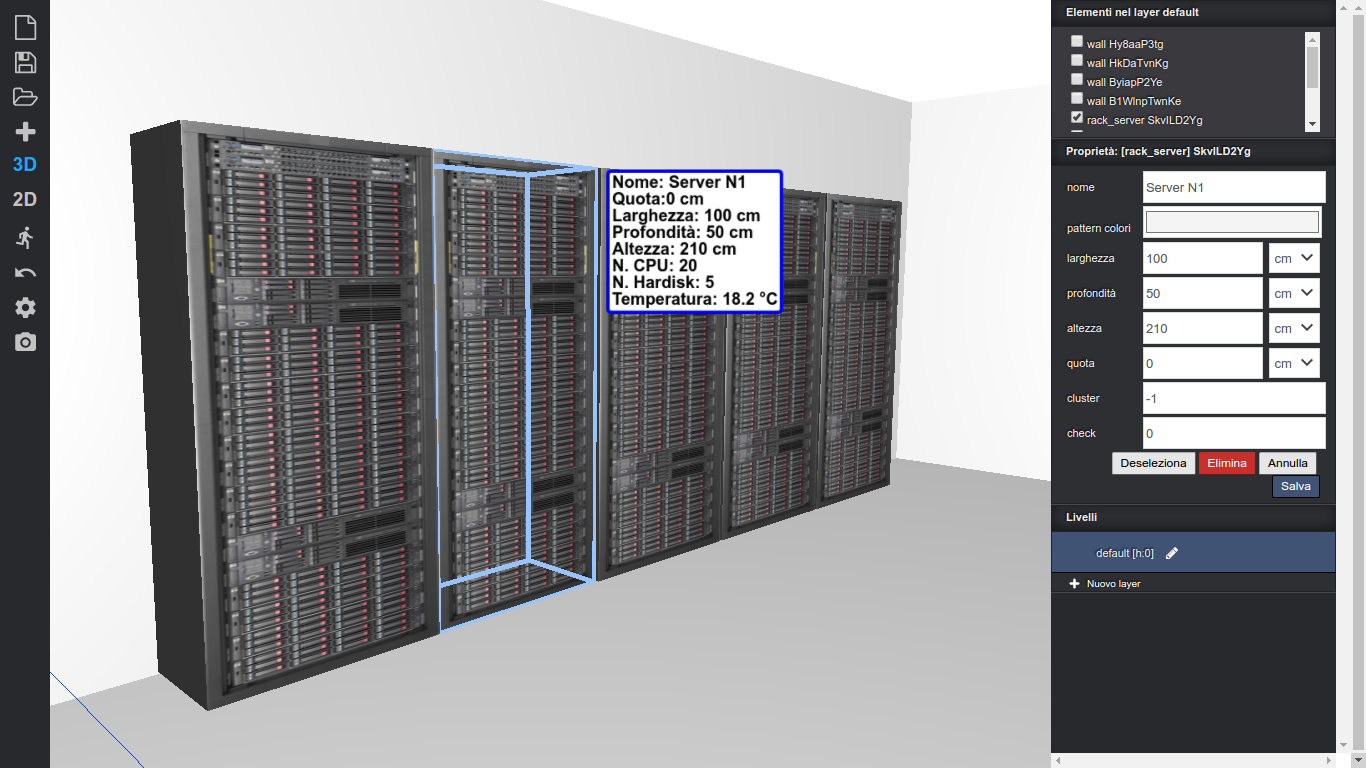
\includegraphics[width=1\linewidth]{images/iot}
   \caption{Plugin con informazioni IoT visualizzate in real-time}
   \label{fig:iot}
   \end{figure}

\newpage

\subsection{Progettazione Collaborativa}
\label{sec:conclusions_section_2_sub_2}
Un altro possibile sviluppo del framework è l'aggiunta della modalità di \emph{Progettazione Collaborativa}, consentendo a più utenti
di collaborare contemporaneamente su uno stesso progetto, ottimizando i tempi di lavoro.
I software proposti per implementare questa funzionalità sono:
\emph{Firebase} e \emph{jsondiff}.\\
\emph{Firebase}~\cite{firebase} è una piattaforma mobile e per applicazioni web con strumenti e infrastrutture progettati
per aiutare gli sviluppatori a creare applicazioni di alta qualità. Si è scelto di utilizzare
il Database Realtime di Firebase  il quale è un database cloud-hosted. I dati vengono memorizzati come JSON e
sincronizzati in tempo reale ad ogni client connesso. Quando si crea applicazioni cross-platform con
tecnologie Android, iOS SDK, e JavaScript, tutti i client condividono una istanza in tempo reale del
database e ricevono automaticamente gli aggiornamenti con i dati più recenti.
Esso è stato scelto per implementare un possibile sistema di autenticazione degli utenti,
fare un controllo degli accessi e dei permessi sul progetto.\\
Si è deciso inoltre di utilizzare il gestore di pacchetti e moduli \emph{npm}~\cite{npm} il quale rende facile agli sviluppatori
JavaScript condividere e riutilizzare il codice e rendendolo facile da aggiornare.
Un \emph{pacchetto} è un file o una directory con uno o più file in essa contenuti, che viene descritto tramite un file chiamato ``package.json''
contenete i metadati del pacchetto stesso. Una tipica applicazione, ad esempio un sito web, può dipendere da decine o centinaia di pacchetti.
Questi pacchetti sono spesso piccoli. L'idea generale è che si crea un piccolo blocco di istruzioni che risolve un problema.
In questo modo è possibile risolvere un problema più grande, attraverso una composizione personalizzata di questi piccoli
blocchi condivisi.
\newpage

Si è scelto il modulo \emph{jsondiff} fornito da \emph{npm}, il quale consente di confrontare nel contesto collaborativo
i file JSON su cui lavorono gli utenti per trovare le modifiche apportate.\\

\noindent
\begin{minipage}{.45\textwidth}
\begin{lstlisting}[
                   numbers=left,
                   frame=trBL,
                   basicstyle=\tiny,
                   caption={JSON originario prima della modifica di un utente},
                   label=struttura]
   ...

   "items": {
     "BkrJVNl9e": {
       "id": "BkrJVNl9e",
       "prototype": "items",
       "type": "cattedra",
       "properties": {
         "altitude": {
           "length": 0,
           "unit": "cm"
         }
       },
       "selected": false,
       "x": 452.23424450039795,
       "y": 1750.8919038286344,
       "rotation": 0
     },
     "Hk1xEVg5g": {
       "id": "Hk1xEVg5g",
       "prototype": "items",
       "type": "banco",
       "properties": {
         "altitude": {
           "length": 0,
           "unit": "cm"
         }
       },
       "selected": false,
       "x": 444.0737738367833,
       "y": 1555.0406079018835,
       "rotation": 0
     }
   },

   ...
\end{lstlisting}
\end{minipage}\hfill
\begin{minipage}{.45\textwidth}
\begin{lstlisting}[
                   numbers=left,
                   frame=trBL,
                   basicstyle=\tiny,
                   caption={JSON dopo la modifica di un utente},
                   label=struttura]
   ...

   "items": {
     "BkrJVNl9e": {
       "id": "BkrJVNl9e",
       "prototype": "items",
       "type": "cattedra",
       "properties": {
         "altitude": {
           "length": 0,
           "unit": "cm"
         }
       },
       "selected": false,
       "x": 452.23424450039795,
       "y": 1750.8919038286344,
       "rotation": 0
     },
     "rkiM4Ngcl": {
       "id": "rkiM4Ngcl",
       "prototype": "items",
       "type": "estintore",
       "properties": {
         "altitude": {
           "length": 100,
           "unit": "cm"
         }
       },
       "selected": false,
       "x": 831.6984550413513,
       "y": 1620.1209426149287,
       "rotation": 0
     }
   },

  ...
\end{lstlisting}
\end{minipage}
\newpage

\begin{lstlisting}[
                   numbers=left,
                   frame=trBL,
                   basicstyle=\tiny,
                   caption={Output dopo l'esecuzione del modulo jsondiff con le differenze tra i due file JSON precedenti},
                   label=struttura]
 layers:
  layer-1:
    items:
      Hk1xEVg5g:
        -
          id:         Hk1xEVg5g
          prototype:  items
          type:       banco
          properties:
            altitude:
              length: 0
              unit:   cm
          selected:   false
          x:          444.0737738367833
          y:          1555.0406079018835
          rotation:   0
        - 0
        - 0
      rkiM4Ngcl:
        -
          id:         rkiM4Ngcl
          prototype:  items
          type:       estintore
          properties:
            altitude:
              length: 100
              unit:   cm
          selected:   false
          x:          831.6984550413513
          y:          1620.1209426149287
          rotation:   0
\end{lstlisting}

Sfruttando le tecnologie sopra descrite, si può pensare di sviluppare il framework \emph{Metior}
per la Progettazione Collaborativa gestendo le modifiche apportate dai diversi utenti che lavorano su uno
stesso progetto seguendo un workflow simile a quello che usa GitHub nella gestione dei repository,
consentendo all'utente di effettuare operazioni come merge, push e pull.
Per gestire il problema della conflittualità sulle modifiche apportate dagli utenti,
si potrebbe inserire una gestione intelligente dei layer consentendo all'utente di fare un ``lock'' sul layer sul quale
sta lavorando non consentendo cosi agli altri utenti di apportare modifiche fino al suo rilascio.
\newpage

\subsection{Fotorealismo}
\label{sec:conclusions_section_2_sub_3}
Con \emph{Fotorealismo} si intende semplicemente che una scena simulata \`e indistinguibile da una fotografia, o per estensione
dalla vita di tutti i giorni. Questo è possibile attraverso un processo di \emph{rasterizzazione}, che consiste in un algoritmo che
permette di convertire un'immagine a due dimensioni in una formata da pixel per avere fotogrammi proiettabili sugli schermi.

Il servizio \emph{Baking}~\cite{baking} \`e un servizio remoto che prende una rappresentazione della scena in JSON come input,
calcola le texture lightmapped, le Mappe Ambientali per riflessione e rifrazione e memorizza le informazioni grafiche
in un formato che \`e compatibile con quello d'ingresso.\\

\begin{figure}[htbp] %  figure placement: here, top, bottom, or page
   \centering
   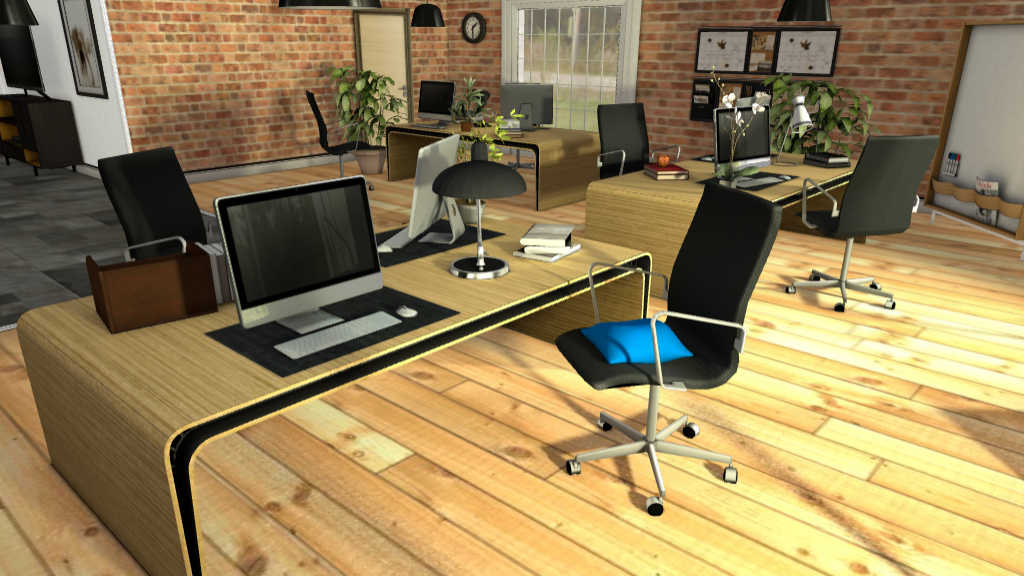
\includegraphics[width=1\linewidth]{images/explorer-a-1}
   \caption{Esempio di un ambiente realizzato con il fotorealismo}
   \label{fig:revit}
   \end{figure}

Lo scopo principale \`e semplificare il workflow durante la visualizzazione 3D per fornire una \emph{User Experience}
ad alto livello sul browser (desktop, tablet e mobile) o su \emph{wearables} come Google Carboard.
\newpage
Lo scopo di questo sviluppo è compattare le strutture dati 3D prodotte dall'editor sul browser, trasmetterle ad un servizio di baking web remoto,
e restituire una piacevole esperienza VR in real-time con alto realismo e frame rate.

\begin{figure}[htbp] %  figure placement: here, top, bottom, or page
   \centering
   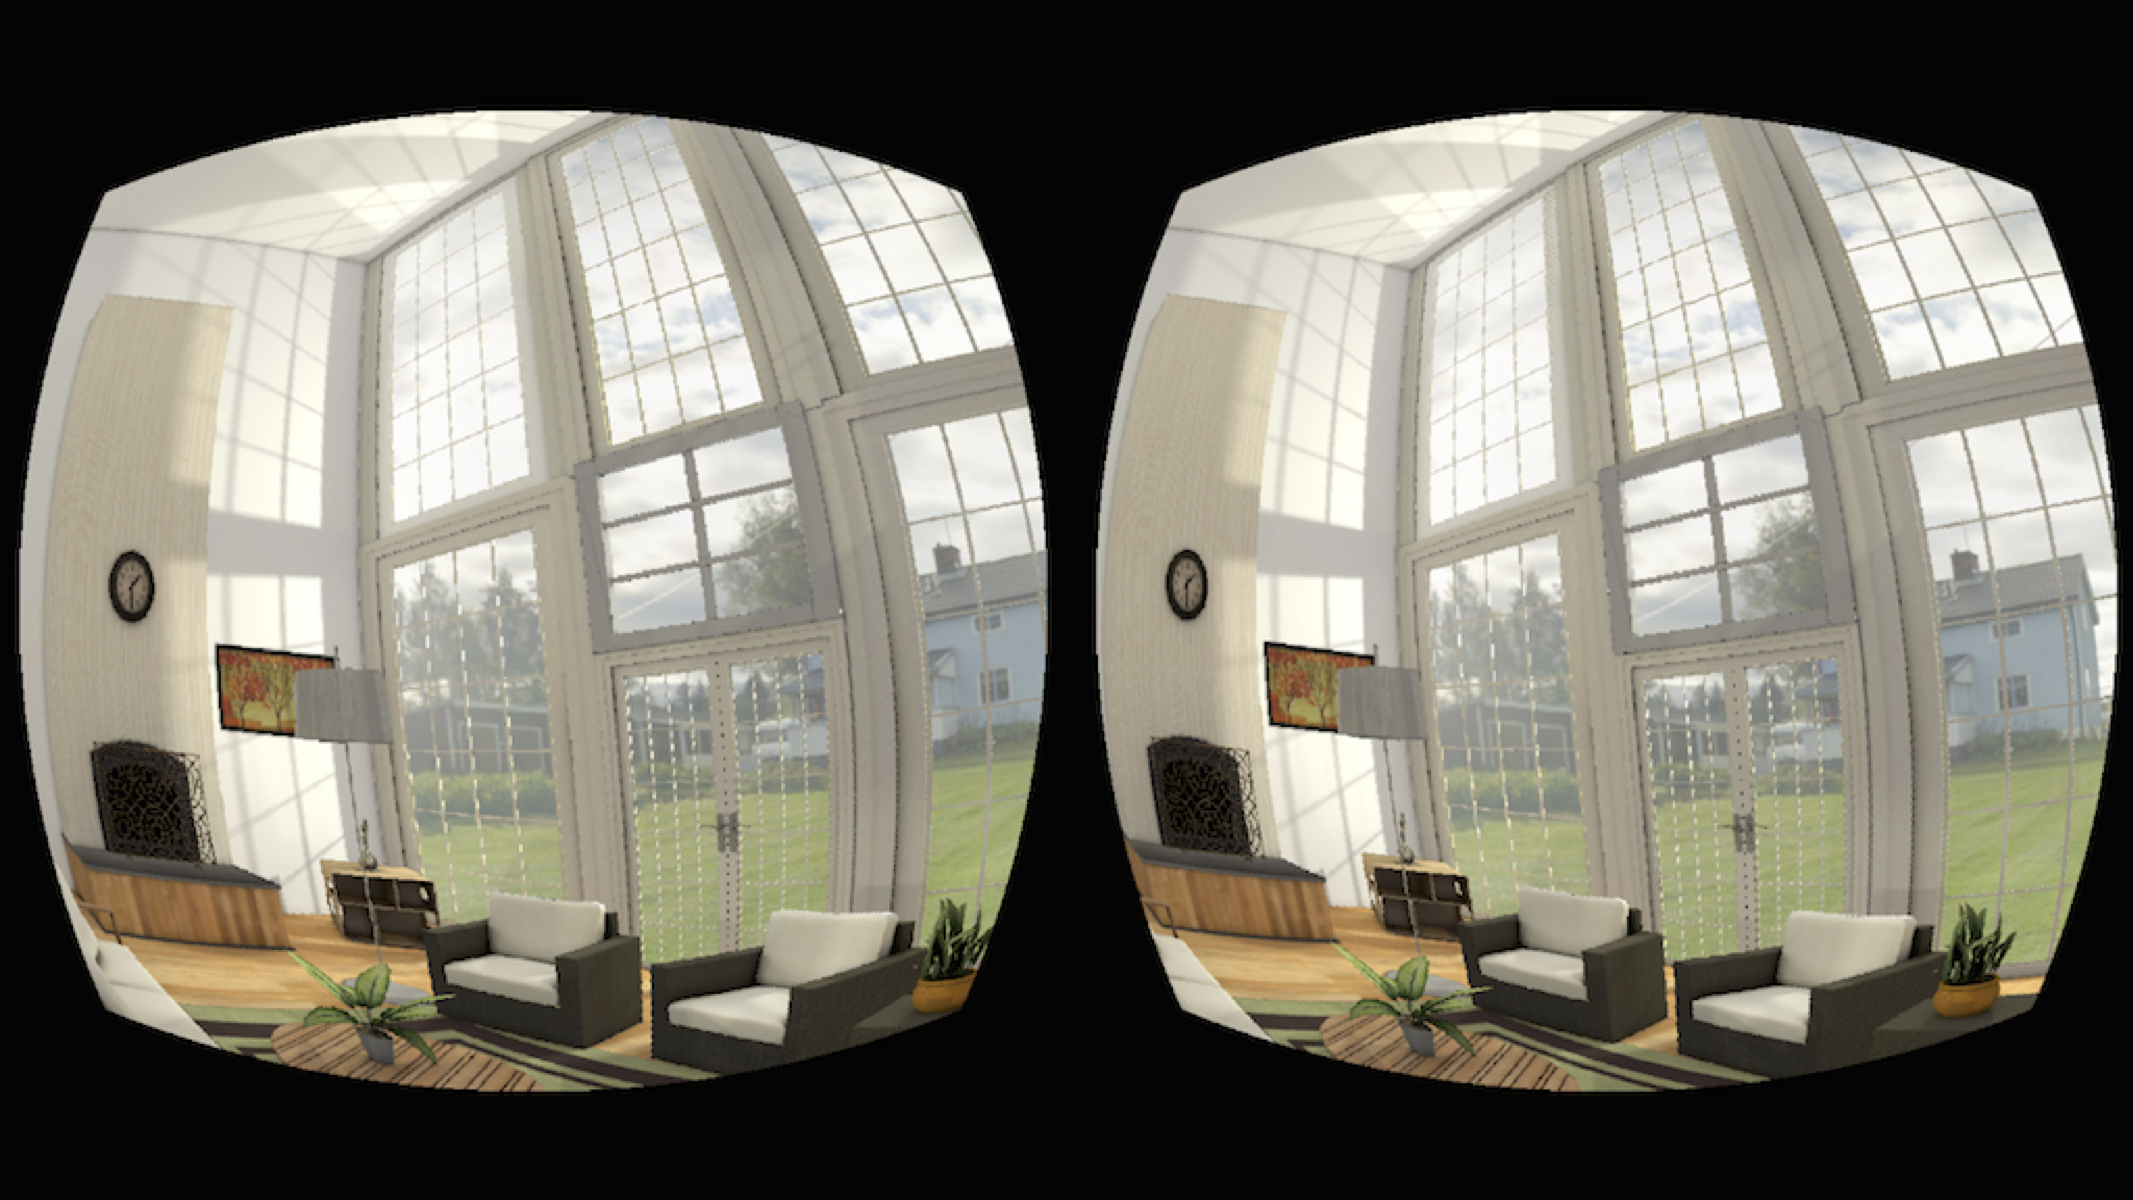
\includegraphics[width=1\linewidth]{images/vr}
   \caption{Esempio di visione di un ambiente attraverso VR}
   \label{fig:revit}
   \end{figure}

Il fotorealismo può essere esteso in un contesto che fornisce Indoor mapping e indoor/outdoor 3D di modelli realistici
partendo da (a) documenti catastali e/o disegni di costruzione, e (b) scansioni outdoor/indoor realizzate tramite droni
che restituiscono un set di fotografie e di nuvole di punti.
